We propose a two-system architecture (Figure~\ref{fig:arch}): a \textbf{prover agent} (System~1) that generates verified proofs through a structured loop, and a \textbf{digest agent} (System~2) that extracts human-learnable knowledge from the proving traces. Lessons from System~2 feed back into System~1 to improve future sessions. Our implementation targets Lean~4 with Mathlib, using an MCP server that exposes a \texttt{check\_lean\_proof} tool for compilation and diagnostics. Source code is available at \url{https://github.com/Ravencus/CS598LMZ-LEAN}.

\begin{figure}[h]
  \centering
  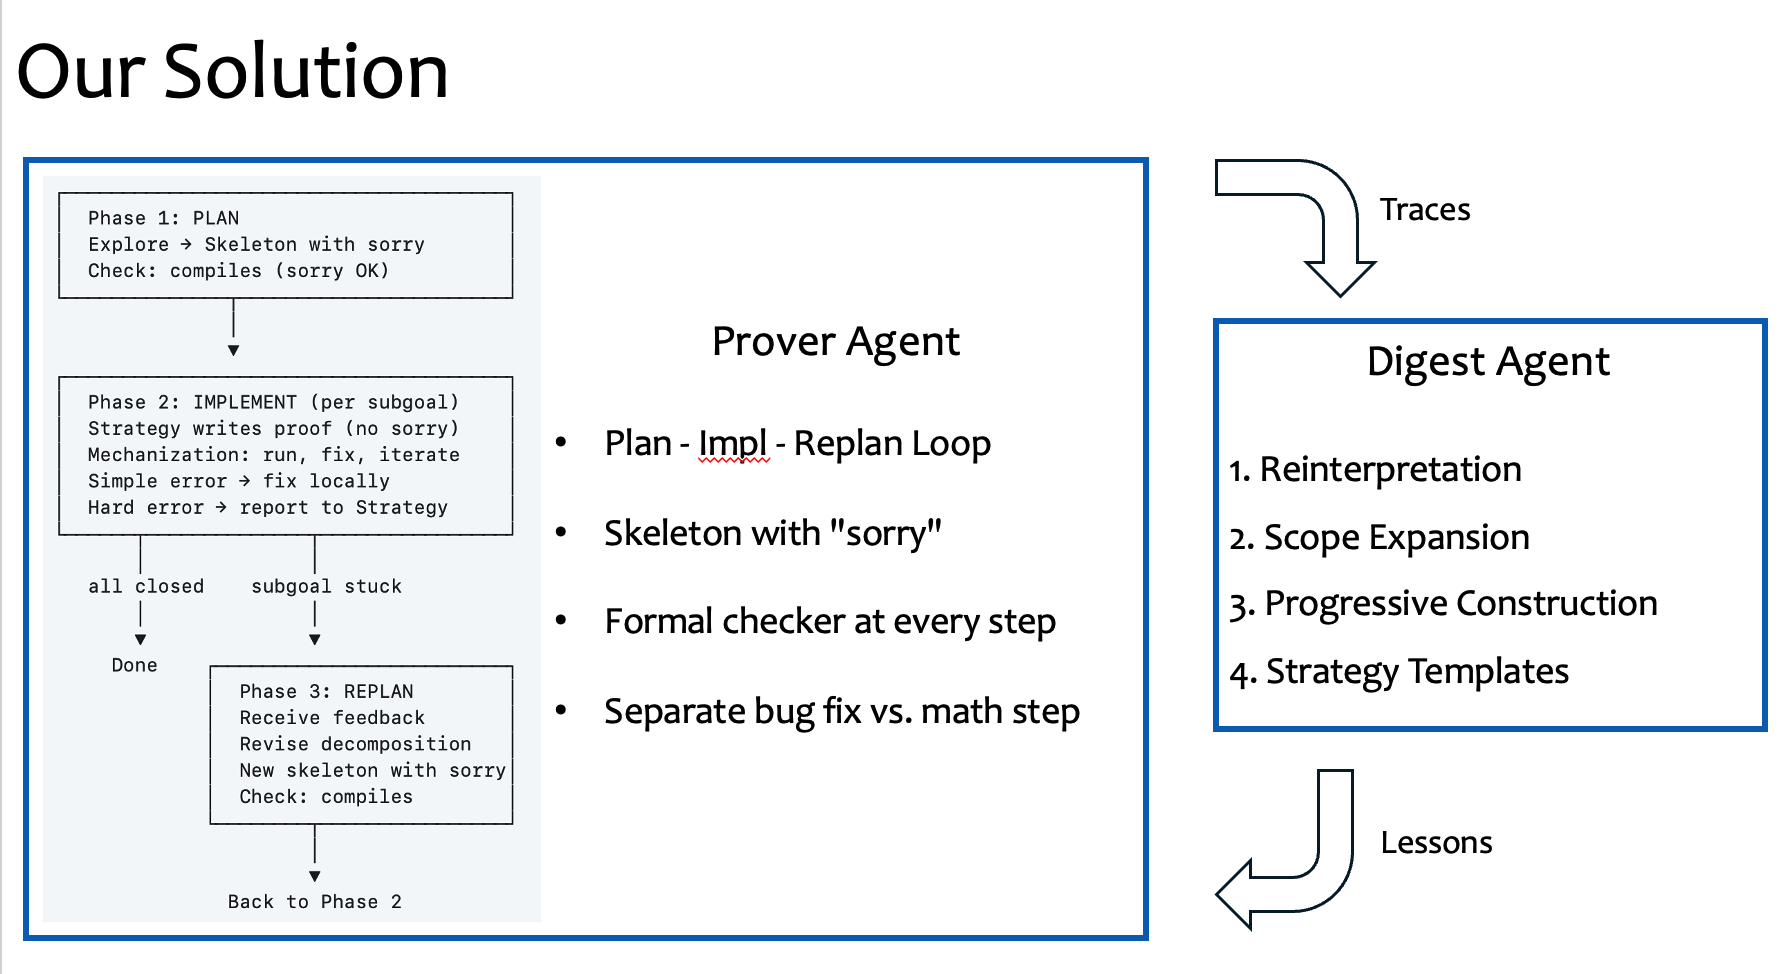
\includegraphics[width=\linewidth]{figures/architecture}
  \caption{Two-system architecture. The prover agent follows a plan--implement--replan loop with proof skeletons. Traces flow to the digest agent, which extracts lessons that feed back to future proving sessions.}
  \label{fig:arch}
\end{figure}

\subsection{System 1: Prover Agent}

The prover operates in three phases. In \textbf{Phase~1 (Plan)}, a strategy agent explores the problem and produces a proof skeleton---a complete Lean file where the main theorem is proved from sorry'd subgoals. The skeleton must compile (sorry warnings are acceptable, errors are not), validating that the decomposition is structurally sound. In \textbf{Phase~2 (Implement)}, each sorry'd subgoal is filled in. A mechanization agent (cheap model with many calls) handles simple compilation errors---wrong lemma names, type mismatches, predicate form issues---and only escalates to the strategy agent (powerful model, few calls) when the error requires mathematical insight. In \textbf{Phase~3 (Replan)}, if a subgoal fails repeatedly, the strategy agent receives structured feedback and revises the decomposition, producing a new skeleton.

\subsection{System 2: Digest Agent}

The digest agent takes a proving trace and performs four core functions that mirror how humans learn from problem-solving. \textbf{Reinterpretation} strips domain-specific surface to find the essential structure (e.g., ``complex numbers'' $\to$ 2D vectors and directional alignment). \textbf{Scope expansion} generates natural follow-up questions that deepen understanding beyond the stated goal (e.g., can we beat $1/6$? what is the optimal bound?). \textbf{Progressive construction} starts from the simplest non-trivial case and identifies what carries forward to the general case. \textbf{Strategy templates} extract high-level approaches and connections to other problems where similar strategies apply. The output is stored as standalone digests and lemma annotations with strategic context, both retrievable by the prover in future sessions.
